% THIS IS SIGPROC-SP.TEX - VERSION 3.1
% WORKS WITH V3.2SP OF ACM_PROC_ARTICLE-SP.CLS
% APRIL 2009
%
% It is an example file showing how to use the 'acm_proc_article-sp.cls' V3.2SP
% LaTeX2e document class file for Conference Proceedings submissions.
% ----------------------------------------------------------------------------------------------------------------
% This .tex file (and associated .cls V3.2SP) *DOES NOT* produce:
%       1) The Permission Statement
%       2) The Conference (location) Info information
%       3) The Copyright Line with ACM data
%       4) Page numbering
% ---------------------------------------------------------------------------------------------------------------
% It is an example which *does* use the .bib file (from which the .bbl file
% is produced).
% REMEMBER HOWEVER: After having produced the .bbl file,
% and prior to final submission,
% you need to 'insert'  your .bbl file into your source .tex file so as to provide
% ONE 'self-contained' source file.
%
% Questions regarding SIGS should be sent to
% Adrienne Griscti ---> griscti@acm.org
%
% Questions/suggestions regarding the guidelines, .tex and .cls files, etc. to
% Gerald Murray ---> murray@hq.acm.org
%
% For tracking purposes - this is V3.1SP - APRIL 2009

\documentclass{acm_proc_article-sp}

\begin{document}

\title{Non-hierarchical Social Learning via Reward-Based Update Filtering}
%
% You need the command \numberofauthors to handle the 'placement
% and alignment' of the authors beneath the title.
%
% For aesthetic reasons, we recommend 'three authors at a time'
% i.e. three 'name/affiliation blocks' be placed beneath the title.
%
% NOTE: You are NOT restricted in how many 'rows' of
% "name/affiliations" may appear. We just ask that you restrict
% the number of 'columns' to three.
%
% Because of the available 'opening page real-estate'
% we ask you to refrain from putting more than six authors
% (two rows with three columns) beneath the article title.
% More than six makes the first-page appear very cluttered indeed.
%
% Use the \alignauthor commands to handle the names
% and affiliations for an 'aesthetic maximum' of six authors.
% Add names, affiliations, addresses for
% the seventh etc. author(s) as the argument for the
% \additionalauthors command.
% These 'additional authors' will be output/set for you
% without further effort on your part as the last section in
% the body of your article BEFORE References or any Appendices.

\numberofauthors{2} %  in this sample file, there are a *total*
% of EIGHT authors. SIX appear on the 'first-page' (for formatting
% reasons) and the remaining two appear in the \additionalauthors section.
%
\author{
% You can go ahead and credit any number of authors here,
% e.g. one 'row of three' or two rows (consisting of one row of three
% and a second row of one, two or three).
%
% The command \alignauthor (no curly braces needed) should
% precede each author name, affiliation/snail-mail address and
% e-mail address. Additionally, tag each line of
% affiliation/address with \affaddr, and tag the
% e-mail address with \email.
%
% 1st. author
\alignauthor
Wesley Tansey\\
       \affaddr{Dept. of Computer Science, The University of Texas at Austin}\\
       \affaddr{1 University Station C0500, Austin, TX, USA}\\
       \email{tansey@cs.utexas.edu}
\alignauthor
Eli Feasley\\
       \affaddr{Dept. of Computer Science, The University of Texas at Austin}\\
       \affaddr{1 University Station C0500, Austin, TX, USA}\\
       \email{elie@cs.utexas.edu}
}
\date{12 December 2011}
% Just remember to make sure that the TOTAL number of authors
% is the number that will appear on the first page PLUS the
% number that will appear in the \additionalauthors section.

\maketitle
\begin{abstract}
Social learning is an extension to Evolutionary Algorithms that enables individuals to learn from observations of others in the population.
 Traditionally, social learning algorithms have employed a student-teacher model where the behavior of one group of individuals is used to train the remaining individuals in the population.  
 We present a non-hierarchical model of social learning in which we do not label each agent, instead allowing any individual which experiences positive reward to teach the rest of the agents on its recent behavior. 
 We validate our approach in a foraging domain, comparing social learning in both Darwinian and Lamarkian paradigms to a standard Darwinian evolution with no learning. 
 We show that our non-hierarchical form facilitates rapid discovery of near-optimal solutions.
\end{abstract}

% A category with the (minimum) three required fields
%\category{D.4.6}{Security and Protection}{Authorization}
%A category including the fourth, optional field follows...
%\category{K.6.5}{Security and Protection}{Authorization}
%\category{E.3}{Data Encryption}{Code breaking}

\terms{Social Learning, Evolutionary Algorithms, Artificial Life}

\section{Introduction}
Biological inspiration
    - Social and Cultural Intelligence Hypotheses
    - Mirror Neurons
        - Reinforcing seen behaviors
    - Learning in primitive communities
    
Summary of approach
    - foraging domain
    - generations of all-new populations
    
Summary of results

Novel contributions
    Non-hierarchical
    Filtering based only on positive rewards
    
Rest of the paper outline
%\begin{itemize}
%\item An improved Markov model capable of more accurately representing a distribution of passwords. 
%\end{itemize}

%The rest of this paper is organized as follows. Section \ref{sec:background} presents background information and related work. Section \ref{sec:model} describes our improved Markov model. Section \ref{sec:evolution} presents our machine learning algorithm for improving a model on-line. Section \ref{sec:results} presents empirical results of our improved model on several real-world datasets and the results of our learning algorithm on a realistic example. Finally, Section \ref{sec:conclusions} presents conclusions and future work.

\section{Non-Hierarchical Social Learning}
\label{sec:nhsl}
Intro
    - Agents acting in parallel
    - Highly expensive simulations
    
Learning from Positive Rewards
    - 1 step memory

Why only positive
    Why backprop works
    Evolution -> avoiding poison

\begin{figure}
  \centering
    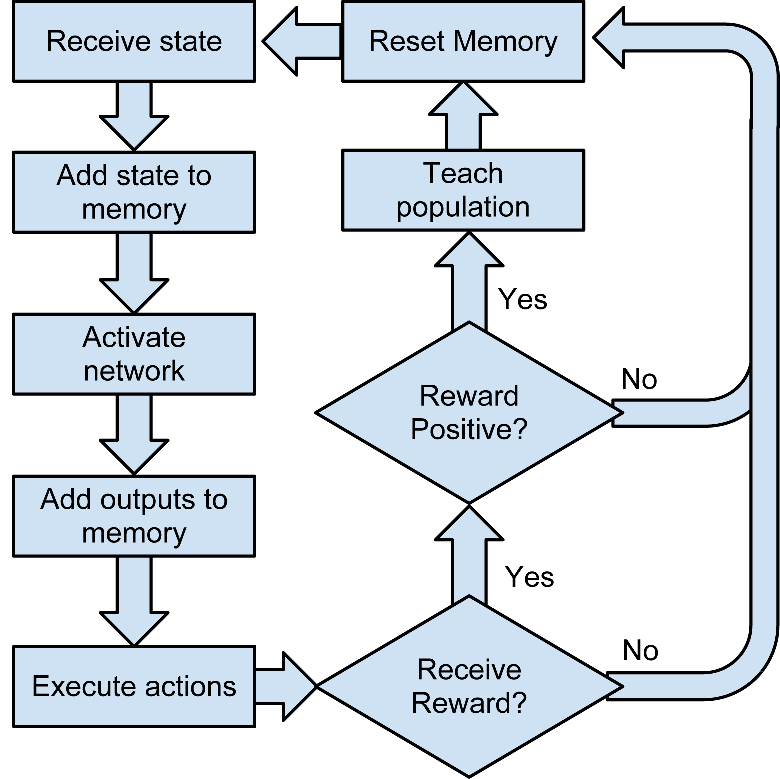
\includegraphics[scale=.6]{flowchart.pdf}
  \caption{FLOWCHART.}
  \label{fig:flowchart}
\end{figure}

\section{Experimental Setup}
\label{sec:setup}

    We use a foraging world in which agents move freely on a continuous toroidal surface which is 500 by 500 units.  
We populate our world with five types of plants - one with a strong reward, one with a weak reward, one which is neutral,one which deals a small penalty to an agent that eats it, and one that deals a large penalty.  
These plants are randomly distributed over the surface of the world.
  The domain is non-competitive and non-cooperative - each agent acts independently of all other agents.
  Each individual begins each generation in the center of the world, with a uniform orientation.
  The plants are randomly distributed around the world, and each individual has 1000 time steps in which to move and consume plants.
  Each plant has a radius of 5 units, and is eaten by any agent that comes within that radius and has not yet eaten the plant (each agent can only eat each plant once, and can only see plants it has not eaten.)
  
 The agents detect plants by means of sensors - they have 8 sensors for each plant, each of which covers 22.5 degrees, leading to a field of view of 180 degrees in front of them.
   They also have a sensor by which they can detect their current velocity.
   These sensors constitute the inputs to the neural network, and the individual's state.
Each agent has two effectors by which it can influence its position - one that controls $\delta v$, the change in velocity, and another that controls $\delta \theta$, the change in angle.
Each of these is one output node of a neural network.
  $\delta v$ is capped between -1 and 1 (the agents can speed up or slow down by one unit per timestep).
  $\delta \theta$ is capped between -30 and 30 degrees, the amount an agent can turn in a timestep.
  The maximum velocity of an agent is 5 units per timestep.
\subsection*{NEAT and SharpNEAT}
NEAT, the NeuroEvolution of Augmented Topologies algorithm for evolving neural networks, was the framework in which we performed our experiments.  
We used NEAT to generate a population of individuals to navigate the world.  
Each individual moving in the world is generated by a genome produced by NEAT, and the fitness of an individual is equal to the sum of all of the plants it eats in a generation (1000 timesteps).
NEAT then uses the fitnesses of these individuals to create new networks by modifying weights and adding and removing connections.

Because NEAT evolves recurrent neural networks, we used backpropagation through time to do our social learning \cite{somedude}.
In Social Darwinian learning and Social Lamarkian learning, we backprop on other individuals whenever an individual receives reward.
In Social Darwinism, as in Darwinan evolution in reality, the changes to the genome do not regress back to the phenome, and the offspring of an individual is determined by the phenome it had before it began learning.
In Social Lamarkism, the changes to the genome as the individual learns are propagated back to the phenome, and the offspring of an individual incorporate what that individual has learned in its lifetime into their phenomes.
\subsection*{Experiments} 
We ran several different experiments to investigate the effect of our approach.
We ran evolution using NEAT both with social learning - both Lamarkian and Darwinian - and without it.
We ran an experiemtn in which we compared learning with all agents sharing information with all other agents to learning with agents only sharing information with other agents in their own species.
In each of these, we kept the size of the world stable at $500\times500$, and the population of agents constant at 100, with 10 different species. 
 We populated the world with 100 plants of varying reward such that the maximum reward is 3000 and the minimum reward is -3000.

\section{Results}
\label{sec:results}
\subsection*{ Baseline, Social Darwin, Social Lamark}
        - Lamarkian quickly reaches a near-optimal solution
        
        - Lamarkian degrades over time after peaking in performance
            - Speculation: Backprop results in poor agents ‘supervising’ strong ones
            - Bad behavior gets reinforced in good agents
            
        - Others slowly climb to reach good solutions
        
        - No meaningful difference between Baseline and Social Darwin
            - The plant rewards are static for each type
            - Learning in darwinian evolution useful only in a dynamic environment
            - Baldwin effect
\subsection*{Population-based vs. Species-based}

Graphs!

Bootstrapping
    Rapidly brings population up to Lamarkian max
    Refines with more efficient baseline of NEAT
    
SPECULATION!
    Inflection points may be artifacts of NEAT
    Some of difficulties in Lamarkian evolution may come from Average handling
    Future experiments will remedy

\section{Related Work}
\label{sec:related}

- Behavior spaces and Culture Algorithms (Reynolds)

    - PSO
    - Explicitly maintained repository of cultural rules
    - Trained at the start of the generation
    
    
- Culture only (Denaro)

    - Shows learning can occur without any evolutionary mutation/crossover at all
    
    - Randomly initialized child (student) networks
    
    - Backprop via Student/Teacher at start of every generation
    
    - Select top 20% of individuals at each generation
    
- NEW TIES (Eiden)

    - Artificial Life (foraging)
    
    - Decision Q-Trees
    
    - Student/Teacher with probabilistic example selection and propagation
    
- Nolfi

    - Simulated annealing for embodied agents
    
-de Oca (Inceremental Social Learning/Particle Swarm)
    - Foraging and Function Optimization domains
    - Added agents to system incrementally (Steady State)
    - Q-Learning and PSO (Value-function learning, not policy)
    - Training examples chosen randomly from two individuals


\section{Future Work}
\label{sec:future}

Reward-proportional updating

Comparison to student/teacher models

Dynamic domains

Language (repellants and attractants, howler monkeys)

Predators (co-evolution, fat agents)

Q-Learning comparison (Ability gained per step)

Variable length trajectories (Memory)

\section{Conclusions}
\label{sec:conclusions}
Summary
Hopeful and uplifting ending

%
% The following two commands are all you need in the
% initial runs of your .tex file to
% produce the bibliography for the citations in your paper.
\bibliographystyle{abbrv}
\bibliography{sigproc}  % sigproc.bib is the name of the Bibliography in this case
% You must have a proper ".bib" file
%  and remember to run:
% latex bibtex latex latex
% to resolve all references
%
% ACM needs 'a single self-contained file'!
%
%APPENDICES are optional
%\balancecolumns
%\appendix
%Appendix A
%\section{Headings in Appendices}
%The rules about hierarchical headings discussed above for
%the body of the article are different in the appendices.
%In the \textbf{appendix} environment, the command
%\textbf{section} is used to
%indicate the start of each Appendix, with alphabetic order
%designation (i.e. the first is A, the second B, etc.) and
%a title (if you include one).  So, if you need
%hierarchical structure
%\textit{within} an Appendix, start with \textbf{subsection} as the
%highest level. Here is an outline of the body of this
%document in Appendix-appropriate form:
%\subsection{Introduction}
%\subsection{The Body of the Paper}
%\subsubsection{Type Changes and  Special Characters}
%\subsubsection{Math Equations}
%\paragraph{Inline (In-text) Equations}
%\paragraph{Display Equations}
%\subsubsection{Citations}
%\subsubsection{Tables}
%\subsubsection{Figures}
%\subsubsection{Theorem-like Constructs}
%\subsubsection*{A Caveat for the \TeX\ Expert}
%\subsection{Conclusions}
%\subsection{Acknowledgments}
%\subsection{Additional Authors}
%This section is inserted by \LaTeX; you do not insert it.
%You just add the names and information in the
%\texttt{{\char'134}additionalauthors} command at the start
%of the document.
%\subsection{References}
%Generated by bibtex from your ~.bib file.  Run latex,
%then bibtex, then latex twice (to resolve references)
%to create the ~.bbl file.  Insert that ~.bbl file into
%the .tex source file and comment out
%the command \texttt{{\char'134}thebibliography}.
%% This next section command marks the start of
%% Appendix B, and does not continue the present hierarchy
%\section{More Help for the Hardy}
%The acm\_proc\_article-sp document class file itself is chock-full of succinct
%and helpful comments.  If you consider yourself a moderately
%experienced to expert user of \LaTeX, you may find reading
%it useful but please remember not to change it.
%\balancecolumns
% That's all folks!
\end{document}
